
\begin{tikzpicture}[line cap=round,line join=round,>=stealth,x=1cm,y=1cm, scale=0.6]
\begin{axis}[
x=1cm,y=1cm,
axis lines=middle,
grid style=dashed,
ymajorgrids=true,
xmajorgrids=true,
xmin=-9,
xmax=9,
ymin=-5,
ymax=5,
xtick={-9,-8,...,9},
ytick={-5,-4,...,5},]
\clip(-9.78,-5.64) rectangle (9.78,5.64);
\draw[line width=2pt,color=blue,smooth,samples=100,domain=-9:1.8] plot(\x,{((\x)-4)/((\x)-2)});
\draw[line width=2pt,color=blue,smooth,samples=100,domain=2.2:9] plot(\x,{((\x)-4)/((\x)-2)});
\draw[color= blue] (-6.6,2.45) node {\Large$f(x) = \dfrac{x-4}{x-2}$};

\end{axis}
\end{tikzpicture}